\documentclass{article}
\usepackage{alltt}
\usepackage{amsfonts}
\usepackage{amsmath}
\usepackage{amssymb}
\usepackage{amsthm}
\usepackage{booktabs}
\usepackage[backend=biber,style=alphabetic]{biblatex}
\usepackage{caption}
\usepackage{enumitem}
\usepackage{fancyhdr}
\usepackage{graphicx}
\usepackage{mathdots}
\usepackage{mathtools}
\usepackage{microtype}
\usepackage[hidelinks]{hyperref}
\usepackage{multirow}
\usepackage{pdflscape}
\usepackage{pgfplots}
\usepackage{siunitx}
\usepackage{textcomp}
\usepackage{slashed}
\usepackage{tabularx}
\usepackage{tikz}
\usepackage{tkz-euclide}
\usepackage[normalem]{ulem}
\usepackage[all]{xy}
\usepackage{imakeidx}
\usepackage[margin=.8in,left=.8in]{geometry}
\usepackage[T1]{fontenc}
\usepackage{lmodern}
\usepackage{cleveref}
%\usepackage{minted}
\usepackage{tikz-cd}

%Theorems

\theoremstyle{definition}
\newtheorem*{aim}{Aim}
\newtheorem*{axiom}{Axiom}
\newtheorem*{claim}{Claim}
\newtheorem*{cor}{Corollary}
\newtheorem*{conjecture}{Conjecture}
\newtheorem*{defi}{Definition}
\newtheorem*{eg}{Example}
\newtheorem*{ex}{Exercise}
\newtheorem*{fact}{Fact}
\newtheorem*{law}{Law}
\newtheorem*{lemma}{Lemma}
\newtheorem*{notation}{Notation}
\newtheorem*{prop}{Proposition}
\newtheorem*{question}{Question}
\newtheorem*{problem}{Problem}
\newtheorem*{rrule}{Rule}
\newtheorem*{thm}{Theorem}
\newtheorem*{assumption}{Assumption}

\newtheorem*{remark}{Remark}
\newtheorem*{warning}{Warning}
\newtheorem*{exercise}{Exercise}

\newtheorem{nthm}{Theorem}[section]
\newtheorem{nlemma}[nthm]{Lemma}
\newtheorem{nprop}[nthm]{Proposition}
\newtheorem{ncor}[nthm]{Corollary}


\renewcommand{\labelitemi}{--}
\renewcommand{\labelitemii}{$\circ$}
\renewcommand{\labelenumi}{(\roman{*})}


% Strike through
\def\st{\bgroup \ULdepth=-.55ex \ULset}


%%%%%%%%%%%%%%%%%%%%%%%%%
%%%%% Maths Symbols %%%%%
%%%%%%%%%%%%%%%%%%%%%%%%%

\let\U\relax
\let\C\relax
\let\G\relax

% Matrix groups
\newcommand{\GL}{\mathrm{GL}}
\newcommand{\Or}{\mathrm{O}}
\newcommand{\PGL}{\mathrm{PGL}}
\newcommand{\PSL}{\mathrm{PSL}}
\newcommand{\PSO}{\mathrm{PSO}}
\newcommand{\PSU}{\mathrm{PSU}}
\newcommand{\SL}{\mathrm{SL}}
\newcommand{\SO}{\mathrm{SO}}
\newcommand{\Spin}{\mathrm{Spin}}
\newcommand{\Sp}{\mathrm{Sp}}
\newcommand{\SU}{\mathrm{SU}}
\newcommand{\U}{\mathrm{U}}
\newcommand{\Mat}{\mathrm{Mat}}

% Matrix algebras
\newcommand{\gl}{\mathfrak{gl}}
\newcommand{\ort}{\mathfrak{o}}
\newcommand{\so}{\mathfrak{so}}
\newcommand{\su}{\mathfrak{su}}
\newcommand{\uu}{\mathfrak{u}}
\renewcommand{\sl}{\mathfrak{sl}}

% Special sets
\newcommand{\C}{\mathbb{C}}
\newcommand{\CP}{\mathbb{CP}}
\newcommand{\GG}{\mathbb{G}}
\newcommand{\N}{\mathbb{N}}
\newcommand{\Q}{\mathbb{Q}}
\newcommand{\R}{\mathbb{R}}
\newcommand{\RP}{\mathbb{RP}}
\newcommand{\T}{\mathbb{T}}
\newcommand{\Z}{\mathbb{Z}}
\renewcommand{\H}{\mathbb{H}}

% Brackets
\newcommand{\abs}[1]{\left\lvert #1\right\rvert}
\newcommand{\bket}[1]{\left\lvert #1\right\rangle}
\newcommand{\brak}[1]{\left\langle #1 \right\rvert}
\newcommand{\braket}[2]{\left\langle #1\middle\vert #2 \right\rangle}
\newcommand{\bra}{\langle}
\newcommand{\ket}{\rangle}
\newcommand{\norm}[1]{\left\lVert #1\right\rVert}
\newcommand{\normalorder}[1]{\mathop{:}\nolimits\!#1\!\mathop{:}\nolimits}
\newcommand{\tv}[1]{|#1|}
\renewcommand{\vec}[1]{\boldsymbol{\mathbf{#1}}}

% not-math
\newcommand{\bolds}[1]{{\bfseries #1}}
\newcommand{\cat}[1]{\mathsf{#1}}
\newcommand{\ph}{\,\cdot\,}
\newcommand{\term}[1]{\emph{#1}\index{#1}}
\newcommand{\phantomeq}{\hphantom{{}={}}}
% Probability
\DeclareMathOperator{\Bernoulli}{Bernoulli}
\DeclareMathOperator{\betaD}{beta}
\DeclareMathOperator{\bias}{bias}
\DeclareMathOperator{\binomial}{binomial}
\DeclareMathOperator{\corr}{corr}
\DeclareMathOperator{\cov}{cov}
\DeclareMathOperator{\gammaD}{gamma}
\DeclareMathOperator{\mse}{mse}
\DeclareMathOperator{\multinomial}{multinomial}
\DeclareMathOperator{\Poisson}{Poisson}
\DeclareMathOperator{\var}{var}
\newcommand{\E}{\mathbb{E}}
\newcommand{\Prob}{\mathbb{P}}

% Algebra
\DeclareMathOperator{\adj}{adj}
\DeclareMathOperator{\Ann}{Ann}
\DeclareMathOperator{\Aut}{Aut}
\DeclareMathOperator{\Char}{char}
\DeclareMathOperator{\disc}{disc}
\DeclareMathOperator{\dom}{dom}
\DeclareMathOperator{\fix}{fix}
\DeclareMathOperator{\Hom}{Hom}
\DeclareMathOperator{\id}{id}
\DeclareMathOperator{\image}{image}
\DeclareMathOperator{\im}{im}
\DeclareMathOperator{\re}{re}
\DeclareMathOperator{\tr}{tr}
\DeclareMathOperator{\Tr}{Tr}
\newcommand{\Bilin}{\mathrm{Bilin}}
\newcommand{\Frob}{\mathrm{Frob}}

% Others
\newcommand\ad{\mathrm{ad}}
\newcommand{\A}{\mathcal{A}}
\newcommand\Art{\mathrm{Art}}
\newcommand{\B}{\mathcal{B}}
\newcommand{\cU}{\mathcal{U}}
\newcommand{\Der}{\mathrm{Der}}
\newcommand{\D}{\mathrm{D}}
\newcommand{\dR}{\mathrm{dR}}
\newcommand{\exterior}{\mathchoice{{\textstyle\bigwedge}}{{\bigwedge}}{{\textstyle\wedge}}{{\scriptstyle\wedge}}}
\newcommand{\F}{\mathbb{F}}
\newcommand{\G}{\mathcal{G}}
\newcommand{\Gr}{\mathrm{Gr}}
\newcommand{\haut}{\mathrm{ht}}
\newcommand{\Hol}{\mathrm{Hol}}
\newcommand{\hol}{\mathfrak{hol}}
\newcommand{\Id}{\mathrm{Id}}
\newcommand{\lie}[1]{\mathfrak{#1}}
\newcommand{\op}{\mathrm{op}}
\newcommand{\Oc}{\mathcal{O}}
\newcommand{\pr}{\mathrm{pr}}
\newcommand{\Ps}{\mathcal{P}}
\newcommand{\pt}{\mathrm{pt}}
\newcommand{\qeq}{\mathrel{``{=}"}}
\newcommand{\Rs}{\mathcal{R}}
\newcommand{\Vect}{\mathrm{Vect}}
\newcommand{\wsto}{\stackrel{\mathrm{w}^*}{\to}}
\newcommand{\wt}{\mathrm{wt}}
\newcommand{\wto}{\stackrel{\mathrm{w}}{\to}}
\renewcommand{\d}{\mathrm{d}}
\renewcommand{\P}{\mathbb{P}}
%\renewcommand{\F}{\mathcal{F}}


\let\Im\relax
\let\Re\relax

\DeclareMathOperator{\area}{area}
\DeclareMathOperator{\card}{card}
\DeclareMathOperator{\ccl}{ccl}
\DeclareMathOperator{\ch}{ch}
\DeclareMathOperator{\cl}{cl}
\DeclareMathOperator{\cls}{\overline{\mathrm{span}}}
\DeclareMathOperator{\coker}{coker}
\DeclareMathOperator{\conv}{conv}
\DeclareMathOperator{\cosec}{cosec}
\DeclareMathOperator{\cosech}{cosech}
\DeclareMathOperator{\covol}{covol}
\DeclareMathOperator{\diag}{diag}
\DeclareMathOperator{\diam}{diam}
\DeclareMathOperator{\Diff}{Diff}
\DeclareMathOperator{\End}{End}
\DeclareMathOperator{\energy}{energy}
\DeclareMathOperator{\erfc}{erfc}
\DeclareMathOperator{\erf}{erf}
\DeclareMathOperator*{\esssup}{ess\,sup}
\DeclareMathOperator{\ev}{ev}
\DeclareMathOperator{\Ext}{Ext}
\DeclareMathOperator{\fst}{fst}
\DeclareMathOperator{\Fit}{Fit}
\DeclareMathOperator{\Frac}{Frac}
\DeclareMathOperator{\Gal}{Gal}
\DeclareMathOperator{\gr}{gr}
\DeclareMathOperator{\hcf}{hcf}
\DeclareMathOperator{\Im}{Im}
\DeclareMathOperator{\Ind}{Ind}
\DeclareMathOperator{\Int}{Int}
\DeclareMathOperator{\Isom}{Isom}
\DeclareMathOperator{\lcm}{lcm}
\DeclareMathOperator{\length}{length}
\DeclareMathOperator{\Lie}{Lie}
\DeclareMathOperator{\like}{like}
\DeclareMathOperator{\Lk}{Lk}
\DeclareMathOperator{\Maps}{Maps}
\DeclareMathOperator{\orb}{orb}
\DeclareMathOperator{\ord}{ord}
\DeclareMathOperator{\otp}{otp}
\DeclareMathOperator{\poly}{poly}
\DeclareMathOperator{\rank}{rank}
\DeclareMathOperator{\rel}{rel}
\DeclareMathOperator{\Rad}{Rad}
\DeclareMathOperator{\Re}{Re}
\DeclareMathOperator*{\res}{res}
\DeclareMathOperator{\Res}{Res}
\DeclareMathOperator{\Ric}{Ric}
\DeclareMathOperator{\rk}{rk}
\DeclareMathOperator{\Rees}{Rees}
\DeclareMathOperator{\Root}{Root}
\DeclareMathOperator{\sech}{sech}
\DeclareMathOperator{\sgn}{sgn}
\DeclareMathOperator{\snd}{snd}
\DeclareMathOperator{\Spec}{Spec}
\DeclareMathOperator{\spn}{span}
\DeclareMathOperator{\stab}{stab}
\DeclareMathOperator{\St}{St}
\DeclareMathOperator{\supp}{supp}
\DeclareMathOperator{\Syl}{Syl}
\DeclareMathOperator{\Sym}{Sym}
\DeclareMathOperator{\vol}{vol}


\addbibresource{aqc.bib}

\crefformat{section}{\S#2#1#3} % see manual of cleveref, section 8.2.1
\crefformat{subsection}{\S#2#1#3}
\crefformat{subsubsection}{\S#2#1#3}

\begin{document}

\title{Topological Quantum Computation}

\author{Jeremias Rieser \\
Advisor: Martin Knudsen}
\date{20.12.2024}

\maketitle

\begin{abstract}
  In order to realize large scale quantum computers, traditional quantum computation suffers from decoherence and will require much more capable methods for error correction than already available \cite{sau_roadmap_2017}. Here we reiterate the ideas starting with \cite{kitaev_fault-tolerant_1997} and \cite{freedman_topological_2002} for building a topologically protected universal set of topological quantum gates using anabelian anyons in a $2 + 1$ dimensional spacetime, and show how they verify DiVincenzo's criteria allowing for universal computation.
\end{abstract}
\medskip
%\tableofcontents


%%%%%%%%%%%%%%%%%%%%%%%%%%%%%%%%%%%%%%%%%%%%
\section{Introduction}
%%%%%%%%%%%%%%%%%%%%%%%%%%%%%%%%%%%%%%%%%%%%

{\it Topological Quantum Computing} (Tqc) was first proposed in 1997 by \cite{kitaev_fault-tolerant_1997}, conjecturing that anyonic braiding could serve as a basis for universal quantum computation. The idea came up in connection with error correcting code, specifically the toric code on a spin lattice model, whose excitations exhibit anyons. This lattice model has since been used to simulate topological quantum computation \cite{satzinger_realizing_2021}.

\subsection{General idea of topological quantum computation}

First, recall the criteria that constitute any classical universal quantum computer:

\begin{enumerate}
  \item Begin by preparing any ground state $\vert \psi \rangle \in (\C^2)^{\otimes n}$.
  \item Then we apply any chain of unitary operators $ \vert \psi \rangle \mapsto U_n \circ U_{n-1} \circ \ldots \circ U_0 \vert \psi \rangle$.
  \item Measure the evolved state.
\end{enumerate}

For topological quantum computation, we claim there is a similar process when considering quasiparticles in $2$ dimensional space. The idea is, that by {\it braiding} the spacetime history of these quasiparticles, we construct a universal gate set. The advantage over classical quantum systems comes from topological protection: The "hidden" information of classical states is {\it topologically protected} as a nonlocal property of the spacetime history.

\subsection{Strategy and outline}
{\bf Outline:}
\begin{itemize}
  \item[{\bf\cref{AnyonsAndTopologicalBerryPhase}}] covers the basics of anyons and their exotic phase behaviour, fusion rules and instantiation and gives an introduction to braid theory.
  \item[{\bf\cref{BraidGatesAndUniversality}}] aims to understand how braid gates can be used to build a set of universal quantum gates, and further how to measure them. More specifically, we show how a {\it linear representation} of the braid group can be used as quantum gates.
  \item[{\bf\cref{Conclusion}}] goes back to our original motivation for constructing this model, namely topological protection, and goes into possible sources of error here and the physical realizability with current methods. We also provide the braid form of our universal basis gates.
\end{itemize}
%%%%%%%%%%%%%%%%%%%%%%%%%%%%%%%%%%%%%%%%%%%%
\section{Anyons and topological (Berry) phase}
\label{AnyonsAndTopologicalBerryPhase}
%%%%%%%%%%%%%%%%%%%%%%%%%%%%%%%%%%%%%%%%%%%%

As motivation for developing this theory, we explore the special properties of $2$ dimensional space, so to say what differentiates $2$ dimensional space from our usual $3$ dimensions. The essential fact we need here, is that in $2$ dimensions, there exists a class of quasiparticles that has fundamentally different properties than those in $3$D.

In quantum mechanics, the state of any system of particles is given by the wavefunction of $N$ particles. As we know, the square modulus of the wavefunction has to be preserved, so any evolution of this state has to be a unitary transformation on the state space. Another property we consider here is the indistinguishability of particles up to position. Furthermore, we do not want any particles occupying the same state, or rather, they should be sufficiently spaced to avoid accidental collisions.
% So to describe our theories mathematically, we define our space of interest as the {\it Configuration space} of $N$ particles living on any space $M$:
%\[
%  Conf_N(M) = \{(x_1,x_2, \ldots ,x_n  ) \in (M)^n \mid x_i \neq x_j \forall i %\neq j  \}
%\]
%Now we want to view an interval in the time evolution of this system, so we view the space $M \times [0,1]$. As we want the state of the particles to be the same on the beginning  (at $t=0$) and the end of the interval ($t=1$) up to their position, we consider the {\it homotopy equivalence classes} $[p] \in \pi_1(Conf_N(M))$ (More on this in \cref{Appendix}). Essentially, we want to project the coordinates of any particle onto a "worldline", so we plot $p(t) \in Conf_M(M)$. Viewing a specific $t$ gives us a slice into space at time $t$.
%
%Mathematically, any unitary transformation $U$ on the wavefunction $\psi(\hat{r})$ of $n$ particles is normally
%\[
%  U\psi(\hat{r}) = \pm \psi(\hat{r})
%\]

In two dimensions, particles can acquire a {\it phase factor} upon exchange, that is not limited to $\pm 1$. Mathematically, the wave function can pick up a phase factor of $e^{i\theta},$\footnote{\label{AnyonName}
 This means, the wave-functions can pick up ``any'' unitary transformation, whence the name Anyon, introduced in \cite{wilczek_quantum_1982}} where $\theta \in [0,\pi]$, so the exchange transformation looks like
\[
  \vert \psi_1 \psi_2 \rangle = e^{i \theta} \vert \psi_2 \psi_1 \ket
\]
In this case, $\theta = 0$ corresponds to bosons {\it (Bose-Einstein statistics)}, and $\theta = \pi$ to fermions {\it (Fermi-Dirac statistics)}. Dealing with anyons results in {\it fractional statistics} \cite{greiter_fractional_2022}\cite{wilczek_quantum_1982}. Furthermore, if we have a non-degenerate ground state \cite{myers_topological_2024}, we can transform by a higher dimensional unitary $U \in U(k)$:
\[
  \vert \psi_1 \psi_2 \rangle = U \vert \psi_2 \psi_1 \rangle
\]
Traditionally, the one dimensional representations are called abelian anyons, while the higher dimensional ones are called anabelian anyons (due to the non-commutativity of unitaries).
Anyons "interpolate" between the FD and BE statistics. In fact, the {\it spin-statistics theorem} asserts that in $3 + 1$ dimensional spacetime, even spin fields are bosonic and half-integer spin fields are fermionic \cite{pauli_connection_1940}.


\vspace{.25cm}



\begin{center}
\begin{tabular}{ll}
\begin{minipage}{9.5cm}
\footnotesize
\noindent
{\bf Figure 1 - The path traced by a particle in the 2 dimensional plane.}  The difference between exchanges in two and three dimensions is more obvious when thinking about it topologically: In three dimensions, any path taken by a particle with the same start and end positions can be deformed into the identity path. However, in two dimensions, a path may trace around another particle, and we cannot contract back to the identity because there is another particle in the way.
\end{minipage}
&
\raisebox{-50pt}{
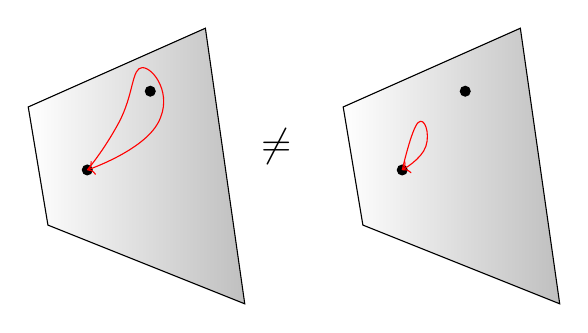
\begin{tikzpicture}

\shade[right color=lightgray, left color=white]
    (2,-1.5) -- (-0.5,-0.5) -- (-0.75,1) -- (1.5,2) -- cycle; 
\draw[]
    (2,-1.5) -- (-0.5,-0.5) -- (-0.75,1) -- (1.5,2) -- cycle;

\fill[black] (0.0, 0.2) circle (2pt);  
\fill[black] (0.8, 1.2) circle (2pt);  

\draw[->, red] plot [smooth, tension=1] coordinates {(0.0, 0.2) (0.4, 0.8) (0.7, 1.5) (0.9, 0.8) (0.0, 0.2)};


\node at (2.4, 0.5) {\Large $\neq$};


\shade[right color=lightgray, left color=white]
    (6,-1.5) -- (3.5,-0.5) -- (3.25,1) -- (5.5,2) -- cycle; 

\draw[]
    (6,-1.5) -- (3.5,-0.5) -- (3.25,1) -- (5.5,2) -- cycle;

    \fill[black] (4.0, 0.2) circle (2pt);  
\fill[black] (4.8, 1.2) circle (2pt);  

\draw[->, red] plot [smooth, tension=1] coordinates {(4.0, 0.2) (4.2, 0.8) (4.3, 0.5) (4.0, 0.2)};

\end{tikzpicture}
}
\end{tabular}{}
\end{center}




Phases around a (potentially closed) loop $\gamma : [0,1] \to  X$ are called {\it Berry phases}, with the properties that under unitary transformations, the eigenspace of the state at the end of the loop is continuously transformable to the eigenspace at the start of the loop \cite{simon_holonomy_1983} \cite{berry_quantal_1984}.

In practice, anyons are mostly seen as (topological) defects propagated by the ground state. As these are solitonic\footnote{\label{Solitonic} If something is solitonic, it has singularities that are preserved under continuous processes on the quantum state}, the time evolutions keep revealing the "defect" properties of the ground state (in the configuration space). But for our paper, thinking of them as (physical) particles is perfectly fine.



%%%%%%%%%%%%%%%%%%%%%%%%%%%%%%%%%%%%%%%%
\subsection{Worldlines and braids}
\label{AnyonInstantiationAndFusion}
%%%%%%%%%%%%%%%%%%%%%%%%%%%%%%%%%%%%%%%%
Perhaps this property becomes even more obvious when we now view the time evolutions process of a pair (or really any number) of anyons, specifically in $2 + 1$ dimensional space-time, so $2$ spacial dimensions view across continuous time intervals. A {\it worldline} is the path traced through time by a single particle living in $2$d space. Generally, in every diagram presented in this paper, the direction of time goes downwards. A group of worldlines is known as a {\it braid}. Generally you can consider a braid as having fixed start and end points, and they can be transformed continuously as long as there is no intersection of braids. Additionally, we don't allow back movements (even if topologically equivalent) as one would have to go back in time.

\begin{figure}[h]
  \centering
  \begin{minipage}{0.3\textwidth}
    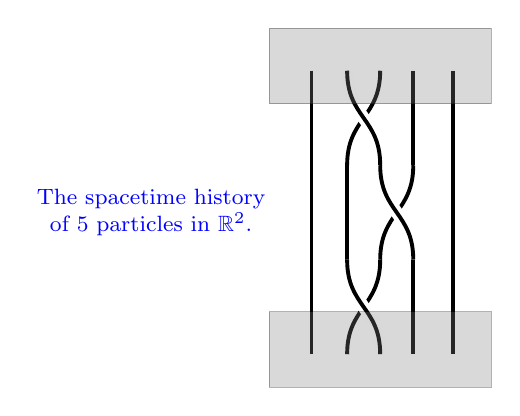
\begin{tikzpicture}
% Squished diagram: scaling the vertical dimension
\begin{scope}[scale=0.6] % Adjust the vertical scaling
  \begin{scope}[shift={(-1.6,0)}]
    \draw[line width=1.2]
      (+.5,5) to (+.5,-1);
  \end{scope}

  \begin{scope}[shift={(0,4)}]
    \draw[line width=1.4]
      (-.35,-1)
      .. controls (-.35,0) and (+.35,0)  ..
      (+.35,1);

    \draw[line width=4.5, white]
      (+.35,-1)
      .. controls (+.35,0) and (-.35,0)  ..
      (-.35,1);
    \draw[line width=1.4]
      (+.35,-1)
      .. controls (+.35,0) and (-.35,0)  ..
      (-.35,1);
  \end{scope}

  \draw[line width=1.4]
    (-.35,3)
    --
    (-.35,1);

  \draw[line width=1.4]
    (+1.05,5)
    --
    (+1.05,3);

  \begin{scope}[shift={(.7,2)}]
    \draw[line width=1.4]
      (-.35,-1)
      .. controls (-.35,0) and (+.35,0)  ..
      (+.35,1);

    \draw[line width=4.5, white]
      (+.35,-1)
      .. controls (+.35,0) and (-.35,0)  ..
      (-.35,1);
    \draw[line width=1.4]
      (+.35,-1)
      .. controls (+.35,0) and (-.35,0)  ..
      (-.35,1);
  \end{scope}

  \begin{scope}
    \draw[line width=1.4]
      (-.35,-1)
      .. controls (-.35,0) and (+.35,0)  ..
      (+.35,1);

    \draw[line width=4.5, white]
      (+.35,-1)
      .. controls (+.35,0) and (-.35,0)  ..
      (-.35,1);
    \draw[line width=1.4]
      (+.35,-1)
      .. controls (+.35,0) and (-.35,0)  ..
      (-.35,1);
  \end{scope}

  \draw[line width=1.4]
    (1.05,1) to (1.05,-1);

  \begin{scope}[shift={(+2.4,0)}]
    \draw[line width=1.4]
      (-.5,5) to (-.5,-1);
  \end{scope}

   % Add baseplate rectangles
  % Top rectangle
  \draw[fill=gray, opacity=0.3] (-2,4.3) rectangle (2.7,5.9);

  % Bottom rectangle
  \draw[fill=gray, opacity=0.3] (-2,-0.1) rectangle (2.7,-1.7);

  \node[align=center, blue, font=\footnotesize] at (-4.5, 2) 
        {The spacetime history \\ of $5$ particles in $\R^2$.};

  \end{scope}
\end{tikzpicture}
  \end{minipage}
  \hfill
  \begin{minipage}{0.3\textwidth}
    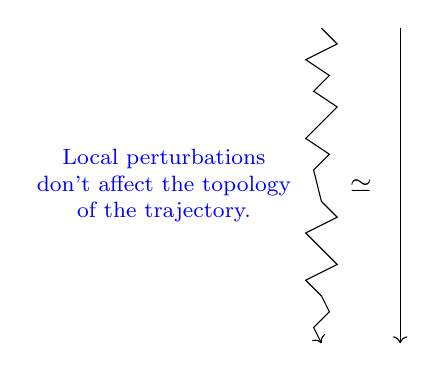
\begin{tikzpicture}
    % Text to the left of the diagram
    \node[align=center, blue, font=\footnotesize] at (-2, 0) 
        {Local perturbations \\ don't affect the topology \\ of the trajectory.};
    
    % Jagged line from top to bottom
    \draw[->] (0,2) -- (0.2,1.8) -- (-0.2,1.6) -- (0.1,1.4) -- (-0.1,1.2)
                 -- (0.2,1) -- (0,0.8) -- (-0.2,0.6) -- (0.1,0.4) -- (-0.1,0.2)
                 -- (0,-0.2) -- (0.2,-0.4) -- (-0.2,-0.6) -- (0,-0.8) 
                 -- (0.2,-1) -- (-0.2,-1.2) -- (0,-1.4) -- (0.1,-1.6) 
                 -- (-0.1,-1.8) -- (0,-2);
    
    % Straight line next to it
    \draw[->] (1,2) -- (1,-2);

    % Isomorphic symbol between the lines
    \node at (0.5, 0) {$\simeq$};
\end{tikzpicture}
  \end{minipage}
  \hfill 
  \begin{minipage}{0.3\textwidth}
    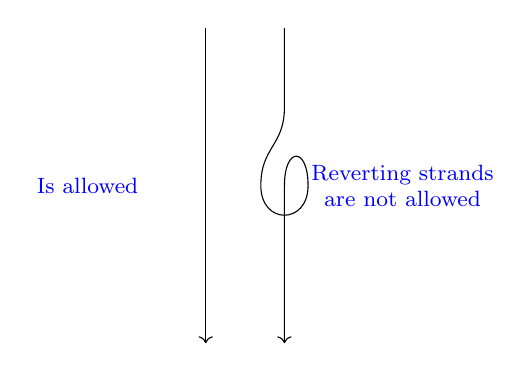
\begin{tikzpicture}
    % Straight line
    \draw[->] (1,2) -- (1,-2);

    % Line with a self-loop
    \draw[->] (2,2) -- (2,1) % Start straight
                 .. controls (2,0.5) and (1.7,0.5) .. (1.7,0) % Loop start
                 .. controls (1.7,-0.5) and (2.3,-0.5) .. (2.3,0) % Bottom of loop
                 .. controls (2.3,0.5) and (2,0.5) .. (2,0) % Loop end
                 -- (2,-2); % Continue straight

    % Labels for clarity
    \node[align = center, blue, font=\footnotesize] at (-0.5,0) {Is allowed};
    \node [align=center, blue, font=\footnotesize] at 
    (3.5,0) {Reverting strands \\ are not allowed};
\end{tikzpicture}

  \end{minipage}
\end{figure}






  










The set of braids has a very well known mathematical group structure. The group action in this case is given by the concatenation of two braids. The basic building block for a braid is given by the two-braid exchange $\sigma_i$ or its inverse $\sigma_i^{-1}$, see Figure 2 \cref{braid:generators}.

\newpage

The {\it braid group} proper is generated by the {\it Artin-Lee} relations given as follows \cite{artin_theory_1950} \cite{fox_braid_1962}:
\begin{align}
  \sigma_i\sigma_j &= \sigma_j\sigma_i, \;\; \left\vert i - j \right\vert \geq 2 \label{eq:al1}\\
  \sigma_i\sigma_{i+1}\sigma_{i} &= \sigma_{i+1}\sigma_i\sigma_{i+1}, \;\; i \in [1,n-2] \label{eq:al2}
\end{align}\label{eq:artin}
where $\eqref{eq:al2}$ is also referred to as the {\it Yang-Baxter equation}. Furthermore, in $3$-dimensions $\sigma_j$ is topologically equivalent to $\sigma_j^{-1}$, as their properties depend on the observers' perspective. So we gain the additional relation $\sigma_j^2 = 1$, which together with $\eqref{eq:al1}$ and $\eqref{eq:al2}$ generates the symmetric group $S_n$. Intuitively, in $3 + 1D$ there are no knots, so a pass under or over does not matter for the topology of the system.


\vspace{0.5cm}

\begin{tabular}{c c c}
  $
\sigma_i
\;\coloneqq\;
\left[
\color{black}
\raisebox{-28pt}{
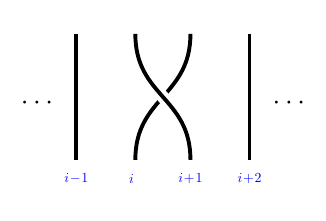
\begin{tikzpicture}[yscale=.8]

\begin{scope}[shift={(-1.6,0)}]
\draw[line width=1.4]
  (+.5,1) to (+.5,-1);
\draw
  (-0,-.1) node {$\mathclap{\cdots}$};
\end{scope}
\draw[line width=1.4]
  (-.35,-1)
  .. controls (-.35,0) and (+.35,0)  ..
  (+.35,1);

\draw[line width=4.5, white]
  (+.35,-1)
  .. controls (+.35,0) and (-.35,0)  ..
  (-.35,1);
\draw[line width=1.4]
  (+.35,-1)
  .. controls (+.35,0) and (-.35,0)  ..
  (-.35,1);
\begin{scope}[shift={(+1.6,0)}]
\draw[line width=1.4]
  (-.5,1) to (-.5,-1);
\draw
  (-0,-.1) node {$\mathclap{\cdots}$};
\end{scope}

\draw
  (-1.1, -1.3) node {\color{blue}\scalebox{.5}{$i\!-\!1$}};
\draw
  (-.4, -1.3) node {\color{blue}\scalebox{.5}{$i$}};
\draw
  (+.35, -1.3) node {\color{blue}\scalebox{.5}{$i\!+\!1$}};
\draw
  (+1.1, -1.3) node {\color{blue}\scalebox{.5}{$i\!+\!2$}};
\end{tikzpicture}
} 
\right]$
&
\begin{minipage}{5.8cm}
\label{braid:generators}
\small
{\bf Figure 2 - Left \& Right: Generators of the braid group.} 
The braid group generators describe the exchanges of adjacent particles. 
The generator $\sigma_i$ represents the $i$-th strand crossing over the $(i+1)$-th strand, while $\sigma_i^{-1}$ represents the inverse process, where the $i$-th strand passes under the $(i+1)$-th strand. The non-crossing strands remain straight. {\bf Bottom: Graphical Yang-Baxter equation} Adapted from \cite{myers_topological_2024}.
\end{minipage}
&
$\sigma_{i}^{-1}
\;\coloneqq \;
\left[
\color{black}
\raisebox{-28pt}{
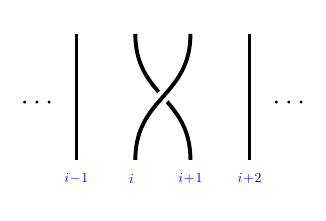
\begin{tikzpicture}[yscale=.8]

\begin{scope}[shift={(-1.6,0)}]
\draw[line width=1.2]
  (+.5,1) to (+.5,-1);
\draw
  (-0,-.1) node {$\mathclap{\cdots}$};
\end{scope}

\draw[line width=1.4]
  (+.35,-1)
  .. controls (+.35,0) and (-.35,0)  ..
  (-.35,1);

\draw[line width=4.5, white]
  (-.35,-1)
  .. controls (-.35,0) and (+.35,0)  ..
  (+.35,1);
\draw[line width=1.4]
  (-.35,-1)
  .. controls (-.35,0) and (+.35,0)  ..
  (+.35,1);

\begin{scope}[shift={(+1.6,0)}]
\draw[line width=1.4]
  (-.5,1) to (-.5,-1);
\draw
  (-0,-.1) node {$\mathclap{\cdots}$};
\end{scope}
\draw
  (-1.1, -1.3) node {\color{blue}\scalebox{.5}{$i\!-\!1$}};
\draw
  (-.4, -1.3) node {\color{blue}\scalebox{.5}{$i$}};
\draw
  (+.35, -1.3) node {\color{blue}\scalebox{.5}{$i\!+\!1$}};
\draw
  (+1.1, -1.3) node {\color{blue}\scalebox{.5}{$i\!+\!2$}};
\end{tikzpicture}
}
\right]
$
\color{black}
\end{tabular}
\color{black}
%%%%%%%%%%%%%%%%%%%%%%%%%%%%%%%%%%%%
%%%%%%%%%%%%%%%%%%%%%%%%%%%%%%%%%%%5

\begin{equation*}
\centering
\label{SecondArtinRelationGraphically}
\color{black}
\left[
\color{black}
\raisebox{-48pt}{
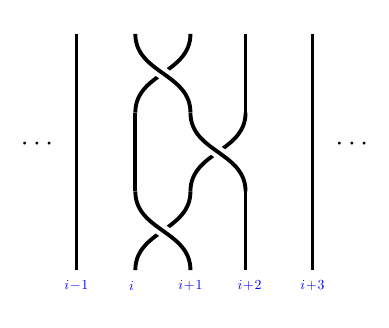
\begin{tikzpicture}[yscale=.5]

\begin{scope}[shift={(-1.6,0)}]
\draw[line width=1.2]
  (+.5,5) to (+.5,-1);
\draw
  (-0,2.2) node {$\mathclap{\cdots}$};
\end{scope}

\begin{scope}[shift={(0,4)}]
\draw[line width=1.4]
  (-.35,-1)
  .. controls (-.35,0) and (+.35,0)  ..
  (+.35,1);

\draw[line width=4.5, white]
  (+.35,-1)
  .. controls (+.35,0) and (-.35,0)  ..
  (-.35,1);
\draw[line width=1.4]
  (+.35,-1)
  .. controls (+.35,0) and (-.35,0)  ..
  (-.35,1);
\end{scope}

\draw[line width=1.4]
  (-.35,3)
  --
  (-.35,1);

\draw[line width=1.4]
  (+1.05,5)
  --
  (+1.05,3);


\begin{scope}[shift={(.7,2)}]
\draw[line width=1.4]
  (-.35,-1)
  .. controls (-.35,0) and (+.35,0)  ..
  (+.35,1);

\draw[line width=4.5, white]
  (+.35,-1)
  .. controls (+.35,0) and (-.35,0)  ..
  (-.35,1);
\draw[line width=1.4]
  (+.35,-1)
  .. controls (+.35,0) and (-.35,0)  ..
  (-.35,1);
\end{scope}


\begin{scope}
\draw[line width=1.4]
  (-.35,-1)
  .. controls (-.35,0) and (+.35,0)  ..
  (+.35,1);

\draw[line width=4.5, white]
  (+.35,-1)
  .. controls (+.35,0) and (-.35,0)  ..
  (-.35,1);
\draw[line width=1.4]
  (+.35,-1)
  .. controls (+.35,0) and (-.35,0)  ..
  (-.35,1);
\end{scope}

 \draw[line width=1.4]
   (1.05,1) to (1.05,-1);

\begin{scope}[shift={(+2.4,0)}]
\draw[line width=1.4]
  (-.5,5) to (-.5,-1);
\draw
  (-0,2.2) node {$\mathclap{\cdots}$};
\end{scope}


\draw
  (-1.1, -1.4) node {\color{blue}\scalebox{.5}{$i\!-\!1$}};

\draw
  (-.4, -1.4) node {\color{blue}\scalebox{.5}{$i$}};

\draw
  (+.35, -1.4) node {\color{blue}\scalebox{.5}{$i\!+\!1$}};

\draw
  (+1.1, -1.4) node {\color{blue}\scalebox{.5}{$i\!+\!2$}};

\draw
  (+1.9, -1.4) node {\color{blue}\scalebox{.5}{$i\!+\!3$}};

\end{tikzpicture}
}
\color{black}
\right]
\color{orange}
\;\;\;\;
=
\;\;\;\;
\color{black}
\left[
\color{black}
\raisebox{-48pt}{
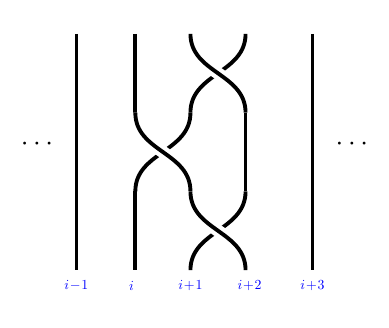
\begin{tikzpicture}[yscale=.5]

\begin{scope}[shift={(-1.6,0)}]
\draw[line width=1.2]
  (+.5,5) to (+.5,-1);
\draw
  (-0,2.2) node {$\mathclap{\cdots}$};
\end{scope}

\begin{scope}[shift={(.7,4)}]
\draw[line width=1.4]
  (-.35,-1)
  .. controls (-.35,0) and (+.35,0)  ..
  (+.35,1);

\draw[line width=4.5, white]
  (+.35,-1)
  .. controls (+.35,0) and (-.35,0)  ..
  (-.35,1);
\draw[line width=1.4]
  (+.35,-1)
  .. controls (+.35,0) and (-.35,0)  ..
  (-.35,1);
\end{scope}


\draw[line width=1.4]
  (1.05,3)
  --
  (1.05,1);

\draw[line width=1.4]
  (-.35,5)
  --
  (-.35,3);


\draw[line width=1.4]
  (-.35,1)
  --
  (-.35,-1);


\begin{scope}[shift={(0,2)}]
\draw[line width=1.4]
  (-.35,-1)
  .. controls (-.35,0) and (+.35,0)  ..
  (+.35,1);

\draw[line width=4.5, white]
  (+.35,-1)
  .. controls (+.35,0) and (-.35,0)  ..
  (-.35,1);
\draw[line width=1.4]
  (+.35,-1)
  .. controls (+.35,0) and (-.35,0)  ..
  (-.35,1);
\end{scope}


\begin{scope}[shift={(.7,0)}]
\draw[line width=1.4]
  (-.35,-1)
  .. controls (-.35,0) and (+.35,0)  ..
  (+.35,1);

\draw[line width=4.5, white]
  (+.35,-1)
  .. controls (+.35,0) and (-.35,0)  ..
  (-.35,1);
\draw[line width=1.4]
  (+.35,-1)
  .. controls (+.35,0) and (-.35,0)  ..
  (-.35,1);
\end{scope}


\begin{scope}[shift={(+2.4,0)}]
\draw[line width=1.4]
  (-.5,5) to (-.5,-1);
\draw
  (-0,2.2) node {$\mathclap{\cdots}$};
\end{scope}

\draw
  (-1.1, -1.4) node {\color{blue}\scalebox{.5}{$i\!-\!1$}};

\draw
  (-.4, -1.4) node {\color{blue}\scalebox{.5}{$i$}};

\draw
  (+.35, -1.4) node {\color{blue}\scalebox{.5}{$i\!+\!1$}};

\draw
  (+1.1, -1.4) node {\color{blue}\scalebox{.5}{$i\!+\!2$}};

\draw
  (+1.9, -1.4) node {\color{blue}\scalebox{.5}{$i\!+\!3$}};

\end{tikzpicture}
}
\color{black}
\right]
\color{black}
\end{equation*}


In the introduction, we mentioned that the braiding is equivalent to the process of applying a unitary evolution.
To show this, we want to relate this braid group $B_n$ to our anyon model defined in \cref{AnyonsAndTopologicalBerryPhase} by choosing a useful {\it linear unitary representation} of our braid group
\[
  \rho : B_n \to U(k)
\]
with emphasis on this representation being of dimension $d > 1$. In 1 dimension, the representation $\rho(\sigma_i) = e^{i\theta} \in \U(1)$ maps every exchange to a complex phase, and in this case our theory is abelian as $\U(1)$ is commutative. Higher dimensional unitaries are non-commutative. As mentioned, we only care about anabelian theories, as they are relevant for computation. Specifically, we will focus on the embedding 
\[
  \rho : B_3 \to U(2),
\]
and the choice for a $3$ particle system will become apparent in \cref{BraidGatesAndUniversality}.




%%%%%%%%%%%%%%%%%%%%%%%%%%%%%%%%
\subsection{Algebraic anyon theory}
\label{FibonacciAnyons}
%%%%%%%%%%%%%%%%%%%%%%%%%%%%%%%%

For the scope of this essay, we will focus on a special case of anabelian anyons, so-called {\it Fibonacci anyons}. This gives us some simplification in the fusion rules and the underlying math, but also is one of the models that allows for universal computation \cite{trebst_short_2008}. In fact, most models from anyons are universal. In any anyonic system there is a particle whose {\it type} (sometimes this is called topological charge) is trivial, and denoted by $1$, constituting the vacuum type (the absence of charge). This trivial particle is its own antiparticle. In order for our fusion rules to be nontrivial, we need at least two different types of anyons. The Fibonacci system uses the trivial type $1$ and the Fibonacci type $\tau$ (Here this is the only "present" type). For our computations, it is sufficient to only consider the type as an abstract concept. Physically, each anyon has a quantum number or a {\it charge}.
%%%%%%%%%%%%%%%%%%%%%%%%%%%%%%
\subsubsection{Fusion}
\label{Fusion}
%%%%%%%%%%%%%%%%%%%%%%%%%%%%%%
For a system of anyons, we define its {\it state} as the set of all possible fusion outcomes, where each outcome defines a state in the Hilbert space of the quantum system \cite{field_introduction_2018}. A single fusion outcome is defined as the {\it group charge}, so the charge remaining after fusing all the anyons in the system.  The dimension of this Hilbert space is equal to the number of possible {\it fusion channels} from an initial system of $n$ anyons to the desired charge ($1$ or $\tau$). For example, we would denote the Hilbert space of $n$ anyons with charge $\tau$ that fuse to $\tau$ by $\mathcal{H}^{\tau^{\otimes n}}_{\tau}$.
{\it Fusion} can be seen as an operation between two particles, forming a new {\it charge}, and similarly, producing a new anyon of one of its possible types. Define $N^{ab}_{c}$ as the number of fusion channels from anyons $x,y$ to charge $z$. For any type of anyon, we define the {\it fusion product} \cite{lahtinen_short_2017} of anyons $a$ and $b$ as 
\[
  a \otimes b = \bigoplus_{o} N^{ab}_{o} o.
\]
For each fusion pair $a \otimes b$, we assign it a vector space $V^{ab}_{c} = \Hom(a\otimes b, c)$, which has dimension $N^{ab}_c$ as above. In fact, for each of these spaces, their $N^{ab}_c$ ways to fuse make up a basis for this space. We can "glue" these spaces if they have appropriate matching indices using the tensor product:


\begin{center}
  \footnotesize{\color{blue}Tensor product $V^{ab}_{x} \otimes V^{xc}_{y}$:}
  \raisebox{-28pt}{
  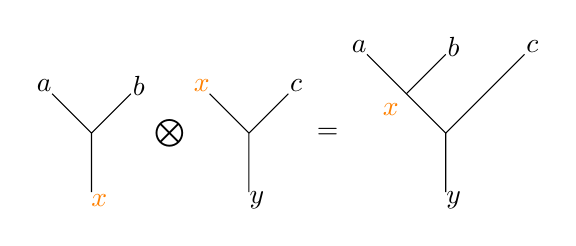
\begin{tikzpicture}
  \centering
  \draw[-] plot coordinates {(0.0, 1.0) (0.5, 0.5) (1.0,1.0) (0.5,0.5) (0.5,-0.25)};
  \node at (1.5, 0.5) {$\bigotimes$};
  \draw [-] plot coordinates {(2.0, 1.0) (2.5,0.5) (3.0,1.0) (2.5,0.5) (2.5,-0.25)};
  \node at (-0.1,1.1) {$a$};
  \node at (1.1,1.1) {$b$};
  \node at (0.6,-0.35) {$\color{orange}x$};
  \node at (1.9,1.1) {$\color{orange}x$};
  \node at (3.1,1.1) {$c$};
  \node at (2.6,-0.35) {$y$};

  \node at (3.5, 0.5) {$=$};

  \draw [-] plot coordinates {(4.0,1.5) (5.0,0.5) (5.0,-0.25)};
  \draw [-] plot coordinates {(6.0,1.5) (5.0,0.5)};
  \draw [-] plot coordinates {(4.5,1.0) (5.0,1.5)};

  \node at (4.3,0.8) {$\color{orange}x$};
  \node at (3.9,1.6) {$a$};
  \node at (5.1,1.6) {$b$};
  \node at (6.1,1.6) {$c$};
  \node at (5.1,-0.35) {$y$};
  %\draw [-] plot coordinates {(1.0,1.0) (0.5, 0.5)};
  %\draw [-]
\end{tikzpicture}}
\end{center}
 

To the fusion of multiple anyons $a^{\otimes n}$ we assign $V^{a^{\otimes n}}_c = \Hom(a^{\otimes n}, c)$, which due to the structure of our space allow for a "nice" decomposition: 
\[
  {V}^{a^{\otimes n}}_{c} = \bigoplus_{c_{1}, \ldots , c_{n-2}  } V^{a_1 a_2}_{{\color{red}c_1}} \otimes V^{{\color{red}c_1} a_3}_{{\color{blue}c_2}} \otimes V^{{\color{blue}c_2} a_4}_{c_3} \otimes \ldots \otimes V^{{c_{n-3}} a_{n-1}}_{\color{orange}c_{n-2}} \otimes V^{{\color{orange}c_{n-2}} a_n}_{c}.
\] (Formally we are operating within a {\it monoidal tensor category} \cite{rowell_mathematics_2017}. These are naturally equipped with the pentagon and hexagon relations in \cref{grp:pentagon} \cite{gelaki_tensor_2015}.) Note that for every fusion space $V^{ab}_{c}$ there exists its dual $V^{c}_{ab}$, called a {\it splitting space}. Splitting occurs, when we lift anyons from a vacuum. To verify that $V^{ab}_{c}$ is an orthonormal basis, we can again use the graphical calculus. Note that we can identify the fusion space with bras and their "time reversal" splitting spaces as a ket. We can immediately verify usual Hilbert space properties:
\begin{figure}[h]
  \centering
    \begin{minipage}{0.45\textwidth}
      \centering
      \color{blue}
      \footnotesize{Inner product $\langle V^{c}_{ab} \vert V_{c^\prime}^{ab} \rangle$:}\\
      \color{black}
      \raisebox{-38pt}{
      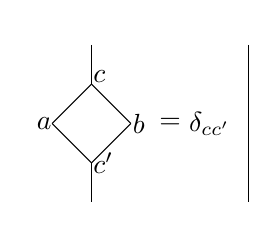
\begin{tikzpicture}
        \node at (0.0, 2.1) {};
        \node at (-0.1, 1.0) {$a$};
        \node at (1.1, 1.0) {$b$}; 
        \draw [-] plot coordinates {(1.0,1.0) (0.5,0.5)};
        \node at (0.6, 1.6) {$c$};
        \draw [-] plot coordinates {(0.0,1.0) (0.5,0.5)};
        \draw [-] plot coordinates {(0.5,0.5) (0.5,0.0)};
        \draw [-] plot coordinates {(0.5,2.0) (0.5, 1.5)};
        \draw [-] plot coordinates {(1.0,1.0) (0.5,1.5)};
        \draw [-] plot coordinates {(0.0,1.0) (0.5, 1.5)};
        \node at (0.65, 0.5) {$c^\prime $};
        \node at (1.5,1.0) {$=$};
        \node at (2.0,1.0) {$\delta_{c c^\prime}$};
        \draw [-] plot coordinates {(2.5,2.0) (2.5, 0.0)};
        \node at (0.0, -0.1) {};
      \end{tikzpicture}}
    \end{minipage}
    \hfill
    \begin{minipage}{0.45\textwidth}
      \centering
      \color{blue}
      \footnotesize{Outer product $\vert V^{ab}_c \rangle \langle V^{c}_{ab} \vert$:}
      \color{black}
      \begin{equation*}
        \sum_{c} 
        \raisebox{-38pt}{
        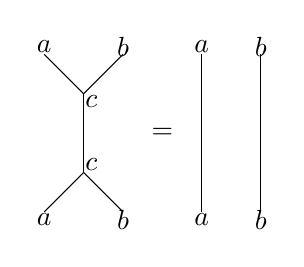
\begin{tikzpicture}
          \node at (0.0, 2.1) {$a$};
          \node at (1.0, 2.1) {$b$};
          \draw [-] plot coordinates {(1.0, 2.0) (0.5, 1.5)};
          \draw [-] plot coordinates {(0.0, 2.0) (0.5, 1.5)};
          \draw [-] plot coordinates {(0.5, 1.5) (0.5, 0.5)};
          \node at (0.0, -0.1) {$a$};
          \node at (1.0, -0.1) {$b$};
          \node at (0.6, 1.4) {$c$};
          \draw [-] plot coordinates {(0.5, 0.5) (1.0, 0.0)};
          \draw [-] plot coordinates {(0.5, 0.5) (0.0, 0.0)};
          \node at (0.6, 0.6) {$c$};
          \node at (1.5,1.0) {$=$};
          \node at (2.0, 2.1) {$a$};
          \node at (2.75, 2.1) {$b$};
          \draw [-] plot coordinates {(2.0,2.0) (2.0,0.0)};
          \draw [-] plot coordinates {(2.75,2.0) (2.75, 0.0)};
          \node at (2.0, -0.1) {$a$};
          \node at (2.75, -0.1) {$b$};
        \end{tikzpicture}}
      \end{equation*}
     
    \end{minipage}
\end{figure}
\vspace{0.5cm}


For the Fibonacci anyons, we can think of the anyon with the vacuum charge $0$ as the absence a particle, so fusion with the vacuum does not change the charge of the other anyon. 
\begin{align*}
  1 \otimes \tau &= \tau \\
  \tau \otimes 1 &= \tau \\
  \tau \otimes \tau &= 1 \oplus \tau
\end{align*}
By $\oplus$ we denote the possibility to result in either outcome. 

To see why these are called Fibonacci anyons, we successively calculate fusion powers of $\tau$:
\begin{align*}
  \tau^{\otimes 3} = \tau \otimes (1 \oplus \tau) 
  &= \tau \oplus (\tau \otimes \tau) 
  = \tau \oplus (1 \oplus \tau) 
  = 1 \oplus 2 \tau \\
  \tau^{\otimes 4} &= 2 \oplus 3\tau \\
  \tau^{\otimes 5} &= 3 \oplus 5\tau \\
  \tau^{\otimes n} &= F_{n+1} \tau \oplus F_{n} 1
\end{align*}
In the case $\tau \otimes \tau$, the probability to fuse to $1$ is $\frac{1}{\phi^2}$ and $\tau$ is $\frac{\phi}{\phi^2}$, where $\phi = \frac{1 + \sqrt{5 } }{2}$. In numbers, these work out to $~38\%$ and $62\%$. The vector space of Fibonacci anyons $V_{\tau^{\otimes n}}^{\tau}$ has dimension $Fib(n)$. Adding a type $1$ anyon to the system does not change the dimension, as all its fusion result on only one outcome. Adding a type $\tau$ anyon however increase the dimension to $Fib(n+1)$. Thus, we define the {\it quantum dimension} of a single anyon in terms of their growth rate towards the entire space, so $dim(1) = 1$ and $dim(\tau) = \lim\limits_{n \to \infty} \frac{Fib(n+1)}{F(n)} = \phi$.


%%%%%%%%%%%%%%%%%%%%%%%%%%%%%%%%
\section{Braid gates and universality}
\label{BraidGatesAndUniversality}
%%%%%%%%%%%%%%%%%%%%%%%%%%%%%%%%

\subsection{Basis of computation}

Using these properties of (anabelian) anyons, we must now construct a basis for our model of computation, with the requirement it is universal. While it may seem convenient to use $\vert (\cdot, \cdot)_{0} \rangle$ and $\vert (\cdot, \cdot)_{\tau} \rangle$ as an orthogonal basis, but this is shown to be rather inconvenient, as we generally want the charge of our space to be conserved. \cite{freedman_topological_2002} \cite{hormozi_topological_2007}. Rather, we initialize each qubit to a three anyon system in a $3$-dimensional Hilbert space. This is done by "pulling" two pairs of anyons form the ground state and discarding the fourth anyon (braiding it away). Our computational basis is made up of $\vert 0 \rangle = \vert ((\cdot,\cdot)_0, \cdot)_{\tau} \rangle$ and $\vert 1 \rangle = \vert ((\cdot,\cdot)_{\tau}, \cdot)_{\tau} \rangle$. The third Hilbert basis is used as a noncomputational state $\vert N \rangle$. Algebraically, we form the computational vector space \cite{ahmadi_zx-calculus_2023}
\[
V^{a_1 a_2 a_3}_{c} = \bigoplus_{d} V^{a_1 a_2}_{{\color{orange}d}} \otimes V^{{\color{orange} d} a_3}_{c}.
\]
For a graphical representation, we draw these qubits to show the fusion order. In all 3 bases, fusion happens from left to right.
\begin{equation*}
  \vert 0 \rangle =
\raisebox{-20pt}{
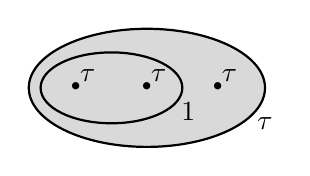
\begin{tikzpicture}[scale=1.5]
    \fill[gray!30] (3,0) ellipse (1 and 0.5);
    \draw[thick] (3,0) ellipse (1 and 0.5);
    
    \draw[thick] (2.7,0) ellipse (0.6 and 0.3);
    \node at (3.35,-0.2) {$1$};
    \node[scale=2.5] at (2.4, 0) {$\cdot$};
    \node at (2.5,0.1) {$\tau$};
    \node[scale=2.5] at (3.0, 0) {$\cdot$};
    \node at (3.1,0.1) {$\tau$};
    \node[scale=2.5] at (3.6, 0) {$\cdot$};
    \node at (3.7,0.1) {$\tau$};
    \node at (4.0,-0.3) {$\tau$};
\end{tikzpicture}
} 
\quad
\vert 1 \rangle = 
\raisebox{-20pt}{
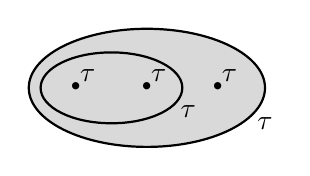
\begin{tikzpicture}[scale=1.5]    
    \fill[gray!30] (3,0) ellipse (1 and 0.5);
    \draw[thick] (3,0) ellipse (1 and 0.5);
    
    \draw[thick] (2.7,0) ellipse (0.6 and 0.3);
    \node at (3.35,-0.2) {$\tau$};

    \node[scale=2.5] at (2.4, 0) {$\cdot$};
    \node at (2.5,0.1) {$\tau$};
    \node[scale=2.5] at (3.0, 0) {$\cdot$};
    \node at (3.1,0.1) {$\tau$};
    \node[scale=2.5] at (3.6, 0) {$\cdot$};
    \node at (3.7,0.1) {$\tau$};
    \node at (4.0,-0.3) {$\tau$};
\end{tikzpicture}
}
\quad 
\vert NC \rangle =
\raisebox{-20pt}{
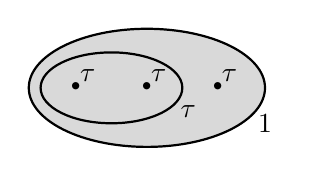
\begin{tikzpicture}[scale=1.5]
    \fill[gray!30] (3,0) ellipse (1 and 0.5);
    \draw[thick] (3,0) ellipse (1 and 0.5);
    
    \draw[thick] (2.7,0) ellipse (0.6 and 0.3);
    \node at (3.35,-0.2) {$\tau$};
    \node[scale=2.5] at (2.4, 0) {$\cdot$};
    \node at (2.5, 0.1) {$\tau$};
    \node[scale=2.5] at (3.0, 0) {$\cdot$};
    \node at (3.1,0.1) {$\tau$};
    \node[scale=2.5] at (3.6, 0) {$\cdot$};
    \node at (3.7,0.1) {$\tau$};
    \node at (4.0,-0.3) {$1$};
\end{tikzpicture}
}
\end{equation*}


\subsection{Braid group representations}

If we talk about a representation $B$ of some structure (category) $A$, we talk about a functor on $B$ with a morphism mirroring the morphism in $A$. Less formally, we try to gain insights about the structure of $A$ in terms of studying (a possibly more familiar) $B$. Here we want to explicitly define the braiding relations given in \cref{AnyonsAndTopologicalBerryPhase} for the aforementioned qubit bases. 


As braiding two anyons in some cases changes the order of fusion, we have to define a change of base for this $3$ dimensional fusion space.
For going from one fusion space decomposition or basis to another, we introduce the $F$-move as a change of base operator. The $F$-move is an isomorphism between fusion spaces \cite{lin_tensor_2020}:
\[
  F^{abc}_{d} : \Hom((a \otimes b) \otimes c, d) \xrightarrow{\sim}  \Hom(a \otimes (b \otimes c), d). 
\]  
and $F^{abc}_{d}$ is in fact an unitary operator on $V_{abc}^d$.
In terms of our vector space decomposition this yields
\[
  F^{abc}_{d} : \bigoplus_{e} V_{e}^{ab} \otimes V_{d}^{ec} \mapsto \bigoplus_{f} V_{d}^{af} \otimes V_{f}^{bc}.
\]  
So we change from a basis in the same space by only considering the inner fusion indices $e$ and $f$. We implicitly assumed that $N_{ab}^{c} \leq 1$ for all spaces, for higher multiplicities we would require an additional index on the $F$ move.
Diagrammatically we can represent this as:
\[
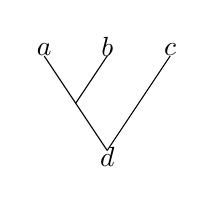
\begin{tikzpicture}[baseline={(current bounding box.center)}, scale=0.8]
  \node at (0,0.1) (a) {$a$};
  \node at (1,0.15) (b) {$b$};
  \node at (2,0.1) (c) {$c$};
  \node at (0.5,-1) (ab) {};
  \node at (1,-1.6) (d) {$d$};
  \draw [-] plot coordinates {(0.0,0.0) (1.0,-1.5)};
  \draw [-] plot coordinates {(1.0,0.0) (0.5,-0.75)};
  %\draw (ab) -- (d);
  \draw [-] plot coordinates {(2.0,0.0) (1.0,-1.5)};
\end{tikzpicture}
\; = \sum_{e} \left[ F_{d}^{abc}\right]_{e}^{f} \;
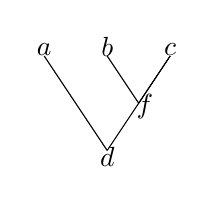
\begin{tikzpicture}[baseline={(current bounding box.center)}, scale=0.8]
  \node at (0,0.1) (a) {$a$};
  \node at (1,0.15) (b) {$b$};
  \node at (2,0.1) (c) {$c$};
  \node at (1.6,-0.8) (bc) {$f$};
  \node at (1,-1.6) (d) {$d$};
  \draw [-] plot coordinates {(1.0,0.0) (1.5,-0.75)};
  \draw [-] plot coordinates {(2.0,0.0) (1.5,-0.75)};
  \draw [-] plot coordinates {(2.0,0.0) (1,-1.5)};
  \draw [-] plot coordinates {(0.0,0.0) (1,-1.5)};
\end{tikzpicture}
\]

Further, as a relation between all our possible basis states, the $F$-move obeys the {\it pentagon equation}, which intuitively means, that any sequence of $F$ moves does not change the final braiding result (or rather the order of fusion does not matter). Note here that the label change is implicitly given as the variables of the sums, and as $F^{abc}_{d}$ is acting on a 3 anyon subspace we have to left or right augment the $F$-moves with the identity operator on a 2 anyon subspace $id_{V^{ab}_{c}}$ 
\begin{center}
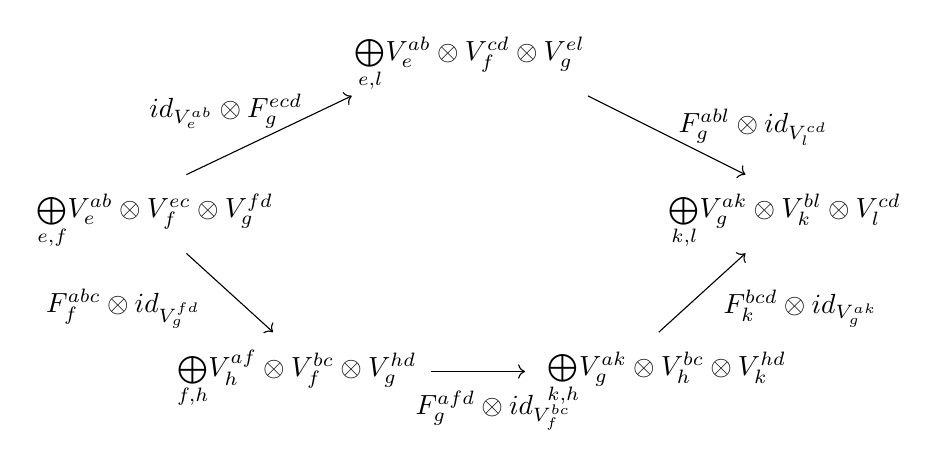
\begin{tikzpicture}
  \node at (0,-0.1) {$\underset{e,f}{\bigoplus} V^{ab}_e \otimes V^{ec}_f \otimes V^{fd}_g $};
  \draw[->, black] plot coordinates{(0.4,0.5) (2.5,1.5)};
  \node at (0.9,1.3) {$id_{V_{e}^{ab}} \otimes F^{ecd}_{g}$};
  \node at (4.0,1.9)  {$\underset{e,l}{\bigoplus} V^{ab}_e \otimes V^{cd}_{f} \otimes V^{el}_g$};
  \node at (7.6, 1.1) {$F^{abl}_{g} \otimes id_{V^{cd}_{l}}$};
  \draw[->] plot coordinates{(5.5, 1.5) (7.5,0.5)};
  \node at (8.0,-0.1) {$\underset{k,l}{\bigoplus} V^{ak}_{g} \otimes V^{bl}_{k} \otimes V^{cd}_{l}$};
  \node at (-0.4, -1.2) {$F^{abc}_{f} \otimes id_{V^{fd}_{g}}$};
  \draw[->] plot coordinates{(0.4,-0.5) (1.5,-1.5)};
  \node at (1.8,-2.1) {$\underset{f,h}{\bigoplus} V^{af}_{h} \otimes V^{bc}_{f}  \otimes V^{hd}_{g}$};
  \node at (4.3, -2.5) {$F^{afd}_{g} \otimes id_{V^{bc}_{f}}$};
  \draw[->] plot coordinates {(3.5,-2.0) (4.7, -2.0)};
  \node at (6.5, -2.1) {$\underset{k,h}{\bigoplus} V^{ak}_{g} \otimes V^{bc}_{h} \otimes V^{hd}_{k} $};
  \node at (8.2, -1.2) {$F^{bcd}_{k} \otimes id_{V^{ak}_{g}}$};
  \draw[->] plot coordinates {(6.4, -1.5) (7.5,-0.5) };
\end{tikzpicture}
\label{grp:pentagon}
\end{center}

For simple theories such as the Fibonacci anyon theory, the pentagon equation suffices to completely determine the $F$ matrix. Furthermore, the {\it MacLane coherence theorem} \cite{mac_lane_categories_1978} guarantees that the pentagon equation is the only "most complicated" constraint on the system. For computation, a purely algebraic expression of the pentagon equation is given as
\[
   \left[ F^{abl}_{g} \right]_{e}^{k} \left[ F^{ecd}_{g} \right]_{f}^{l} = \sum_{h} \left[ F^{bcd}_{k} \right]_{h}^{l} \left[ F^{afd}_{g} \right]_{f}^{k} \left[ F^{abc}_{f} \right]_{e}^{h}.
\]

By direct computation over the pentagon equation we obtain the $F$ matrix for the Fibonacci theory as 
\[
  F^{\tau\tau\tau}_{\tau} := \begin{pmatrix}
    \phi^{-1}  & \phi^{-1 / 2}  \\
    \phi^{-1 / 2} & \phi^{-1}  \\
  \end{pmatrix}.
\]

Now we want to formalize how the particle exchange introduced in \cref{AnyonsAndTopologicalBerryPhase} affects the phase of the qubit. We again introduce a unitary operator, this time we call it the $R$ move, exchanging two particles. Formally, we have $R^{ab}_{c} : V^{ab}_{c} \xrightarrow{\sim} V^{ba}_{c}$. Diagrammatically this is shown as
\begin{center}
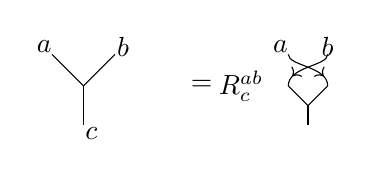
\begin{tikzpicture}[  braid/.style={postaction={decorate}, decoration={markings, mark=at position 0.8 with {\arrow{>}}}},]
  \node at (0.0, 1.0) {$a$};
  \node at (1.0, 1.0) {$b$}; 
  \draw [-] plot coordinates {(0.1,0.9) (0.5,0.5)};
  \draw [-] plot coordinates {(0.9,0.9) (0.5,0.5)};
  \draw [-] plot coordinates {(0.5,0.5) (0.5,0.0)};
  \node at (0.6,-0.1) {$c$};
  \node at (2.0, 0.5) {$=$};
  \node at (2.5, 0.5) {$R^{ab}_{c}$};
  \node at (3.0, 1.0) {$a$};
  \node at (3.6, 1.0) {$b$};
  \draw[braid] (3.1, 0.9) .. controls (3.1, 0.75) and (3.6, 0.75) .. (3.6, 0.5);
  \draw[braid] (3.6, 0.9) .. controls (3.6, 0.75) and (3.1, 0.75) .. (3.1, 0.5);
  \draw[-] plot coordinates {(3.1, 0.5) (3.35, 0.25)};
  \draw[-] plot coordinates {(3.6, 0.5) (3.35, 0.25)};
  \draw[-] plot coordinates {(3.35, 0.25) (3.35, 0.0)};
\end{tikzpicture}
\end{center}

We again constrain the $R$ moves with a commutative diagram similarly to the pentagon equation, but this time we have to mix in $F$ moves. The {\it hexagon equation} is given diagrammatically as
\[
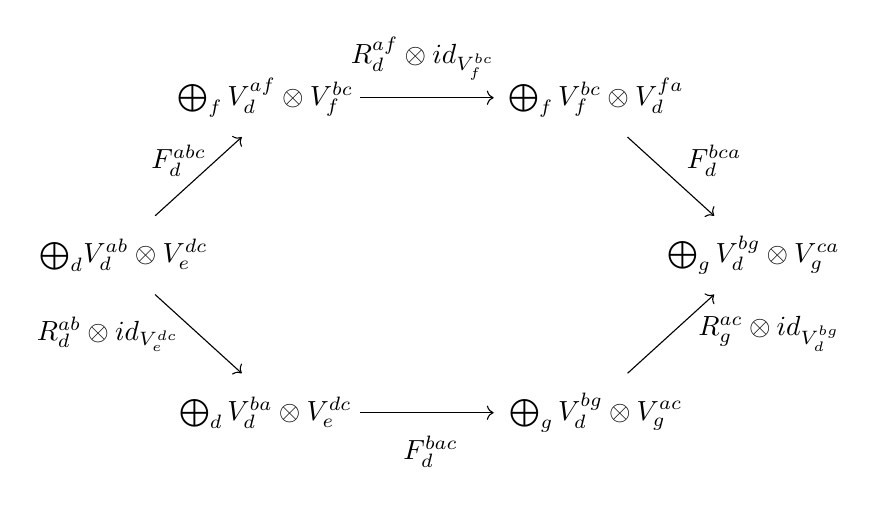
\begin{tikzpicture}
  \node at (0,0) {${\bigoplus}_{d} V^{ab}_d \otimes V^{dc}_{e}$};
  \draw[->, black] plot coordinates{(0.4,0.5) (1.5,1.5)};
  \node at (0.7,1.2) {$F^{abc}_{d}$};
  \node at (1.8,2.0)  {$\bigoplus_{f} V^{af}_{d} \otimes V^{bc}_{f} $};
  \node at (7.5, 1.2) {$F^{bca}_{d} $};
  \draw[->] plot coordinates {(3.0,2.0) (4.7,2.0)};
  \node at (3.8, 2.5) {$R^{af}_{d} \otimes id_{V^{bc}_{f}}$};
  \node at (6.0,2.0) {$\bigoplus_{f} V^{bc}_{f} \otimes V^{fa}_{d}$};
  \draw[->] plot coordinates{(6.4, 1.5) (7.5,0.5)};
  \node at (8.0,0.0) {$\bigoplus_{g} V^{bg}_{d} \otimes V^{ca}_{g} $};
  \node at (-0.2, -1.0) {$R^{ab}_{d} \otimes id_{V^{dc}_{e}}$};
  \draw[->] plot coordinates{(0.4,-0.5) (1.5,-1.5)};
  \node at (1.8,-2.0) {$\bigoplus_{d} V^{ba}_{d} \otimes V^{dc}_{e}$};
  \node at (3.9, -2.5) {$F^{bac}_{d}$};
  \draw[->] plot coordinates {(3.0,-2.0) (4.7, -2.0)};
  \node at (6.0, -2.0) {$\bigoplus_{g} V^{bg}_{d} \otimes V^{ac}_{g}$};
  \node at (8.2, -1.0) {$R^{ac}_{g} \otimes id_{V^{bg}_{d}}$};
  \draw[->] plot coordinates {(6.4, -1.5) (7.5,-0.5) };
\end{tikzpicture}
\label{grp:hexagon}
\]
and algebraically as
\[
  \sum_{f} \left[ F^{abc}_{e} \right]_{d}^{f} \left[ R^{af}_{d} \right] \left[F^{bca}_{d}\right]_{f}^{g} = \left[ R^{ab}_{e} \right] \left[ F^{bac}_{d}\right]_{e}^{g} \left[ R^{ac}_{g}\right]
\]

As the RHS only changes from fixed label $e$ to fixed label $g$, so we do not need to sum over it.
The hexagon equation gives us two necessary components:
\begin{enumerate}
  \item The $F$-move is compatible with the $R$ move (this means we can braid and fuse).
  \item The Yang-Baxter equation \eqref{eq:al2} is fulfilled by the $R$ move.
\end{enumerate}
Similarly to the $F$-move, we can determine the $R$ move by elementary algebra to be
\[
  R \coloneqq \begin{pmatrix}
    e^{\frac{-4\pi i}{5}} & 0  \\
    0 & e^{\frac{3\pi i}{5}}  \\
  \end{pmatrix}
\]

\subsubsection{A note on measurement}

There are multiple ways to measure the result of the braiding. For a general way, we can visualize moving a test particle around the braiding result and observing its interference patterns \cite{simon_topological_2021}. There are also anyon type and hardware specific interferometry methods, introduced by \cite{overbosch_inequivalent_2001} and developed by \cite{bonesteel_braid_2005}.

%%%%%%%%%%%%%%%%%%%%%%%%%%%%%%%%%%%%%%
\subsection{Universal gates}
%%%%%%%%%%%%%%%%%%%%%%%%%%%%%%%%%%%%%%

Now that we have our building blocks in place, we can look at higher dimensional representations of our braid group, specifically $B_3$ as we build $3$ particle qubits. We want our representations of the form
\[
  \varphi : B_3 \to \U(\Hom(a^{\otimes 3}, b))
\]

As we are on a $3$ anyon subspace, there are only four braid generators $\sigma_1, \sigma_2$ and $\sigma_1^{-1}, \sigma_2^{-1}$. Far commutativity is not necessary here, and there is one identity $\sigma_2 \sigma_1 \sigma_2 = \sigma_1 \sigma_2 \sigma_1$ and its inverse relationship. In our basis, the first exchange is trivial, as the leftmost anyons are in the same fusion basis, and thus $\rho(\sigma_1) = R^{ab}_{c}$. The second one is more complicated as we have to braid the results over two bases, but there we can just use a change of base and the hexagon equation like this:
\[
  \rho(\sigma_2) = \left(F^{acb}_{d}\right)^{\dagger}R^{bc}_{d}F^{abc}_{d}
\]

Depending on the literature, the braid operators on the $V^{a a a}_{a}$ basis are sometimes given in $3$ dimensions: 
\begin{align*}
  \rho(\sigma_1) = \begin{pmatrix}
    e^{3\pi i / 5} & 0 & 0  \\
    0 & e^{-4 \pi i / 5}  & 0  \\
    0 & 0 & e^{3\pi i / 5}  \\
  \end{pmatrix}  \text{ and } \quad \rho(\sigma_2) = \begin{pmatrix}
    e^{3\pi i / 5} & 0 &  0 \\
    0 & \phi^{-1} e^{4 \pi i / 5} &  \phi^{-1 / 2} e^{-3 \pi i / 5} \\
    0 & \phi^{-1 / 2}e^{-3 \pi i / 5} & -\phi^{-1}  \\
  \end{pmatrix}
\end{align*}
Recall this acts on the space $(\vert N \rangle, \vert 0 \rangle, \vert 1 \rangle)^T$. So the trivial phase factor (the identity) is applied to the non-computational state. But as we can generally ignore the non-computational state for 1 qubit gates, we can omit tensoring with $id_{V^{aa}_{a}}$, we can stay in two dimensions for our representation as
\[
\rho(\sigma_1) = \begin{pmatrix}
    e^{-4 \pi i / 5}  & 0  \\
    0 & e^{3\pi i / 5}  \\
  \end{pmatrix}  \text{ and } \quad \rho(\sigma_2) = \begin{pmatrix}
    \phi^{-1} e^{4 \pi i / 5} &  \phi^{-1 / 2} e^{-3 \pi i / 5} \\
    \phi^{-1 / 2}e^{-3 \pi i / 5} & -\phi^{-1}  \\
  \end{pmatrix}
\]
\begin{thm}[\cite{freedman_modular_2000}]
  The Fibonacci representation on $V^{\tau^{\otimes 3}}_{\tau}$ is dense in $\U(2)$:
  \[
    \overline{\rho(B_3)} \supset \U(2)
  \]
\end{thm}




\begin{thm}[{\it Universality} in classical quantum computing]\label{ClassicalGateSet}
  In a classical quantum system, the set of gates 
  \[
     \left\{H \coloneqq \frac{1}{\sqrt{2} }\begin{pmatrix}
      1 &  1 \\
      1 &  -1 \\
    \end{pmatrix}, T \coloneqq  \begin{pmatrix}
      1 &  0 \\
      0 &  e^{i \frac{\pi}{4}} \\
    \end{pmatrix}, CNOT \coloneqq  \begin{pmatrix}
      1 & 0 & 0 &  0 \\
      0 & 1 & 0 &  0 \\
      0 & 0 & 0 &  1 \\
      0 & 0 & 1 &  0 \\
    \end{pmatrix}\right\}
  \]
  is universal \cite{brylinski_universal_2001}.
\end{thm}

\section{Conclusion}
\label{Conclusion}
\subsection{Single qubit gates}
We know that the density result is enough to allow universal computation, but as a sanity check we actually want to show a suitable braid representation for the universal set above. As a note, we generally cannot find exact representations of every unitary matrix, but rather approximations with an arbitrarily small error $\epsilon > 0$.

To check this error, we define a norm for unitary $U,V \in \U(D)$ as
\begin{equation}
  dist(U,V) = \sqrt{1 - \frac{\left\vert U^{\dagger} V \right\vert }{D}} \label{eq:norm}
\end{equation}

We can start out with a brute force approach for calculating the two single qubit gates for braids with length at most $n$. 

We define a simple procedure with a target matrix $U_{target} \in \U(2)$, that simply enumerates all $4^n$ possible braids and chooses the best approximation according to \cref{eq:norm}. This found the following braids:
\setcounter{figure}{2}
\begin{figure}[h!]
  \centering
  \begin{minipage}{0.45\textwidth}
    \centering
      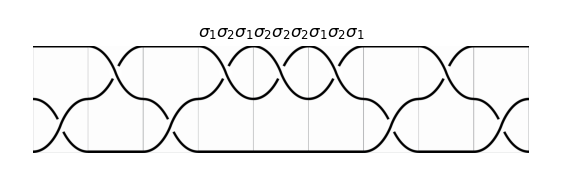
\includegraphics[width=0.8\textwidth]{images/H_braid.png}
      \caption{The braid for the $H$ gate with error 0.05}
      \label{fig:hbraid}
  \end{minipage}
  \hfill
  \begin{minipage}{0.45\textwidth}
      \centering
      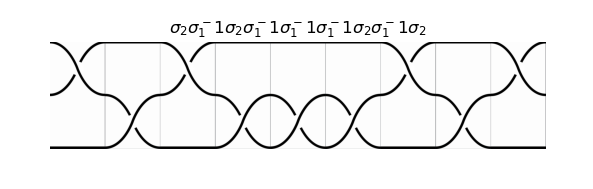
\includegraphics[width=0.8\textwidth]{images/T_braid2.png}
      \caption{The braid for the $T$ gate with error 0.052}
      \label{fig:tbraid}
  \end{minipage}
\end{figure}

Another example for approximating the Pauli $X$ gate $\begin{pmatrix}
  0 &  1 \\
  1 &  0 \\
\end{pmatrix}$ by braids with lengths $5$ and $9$
\begin{align*}
  U_{aprox5} = \sigma_2 \sigma_1^{-3} \sigma_2 &\quad U_{aprox9} = \sigma_1^{-1}\sigma_2\sigma_1^{-1}\sigma_2^{-2}\sigma_1\sigma_2^{-1}\sigma_{1}
\end{align*}
with $dist(X,U_{approx5}) \approx 0.168$ and $dist(X,U_{approx9}) = 0.079$.

This is however very inefficient and  time consuming. Even though there are small optimizations such as using the periodicity of the braid group and excluding inverse operations (as the do nothing for the braid), this is still in exponential time. It turns out however there is an appropriate algorithm called the {\it Solovay-Kitaev} algorithm \cite{bonesteel_braid_2005}\cite{dawson_solovay-kitaev_2005} proposed by Solovay \cite{solovay_email} and proven by kitaev \cite{kitaev_fault-tolerant_1997}. The Solovay-Kitaev algorithm requires a target gate and a desired accuracy $\epsilon $ and returns a braid of length 
\[
  \mathcal{O}\left( \log(1 / \epsilon )^{\frac{\ln(5)}{\ln{3 / 2}}}\right)
\]
with time complexity:
\[
  \mathcal{O}\left( \log(1 / \epsilon )^{\frac{\ln(3)}{\ln{3 / 2}}}\right)
\]
The braid finding problem has started the field of quantum compiling, and there have been found more efficient models and new approaches, e.g. using galois theory \cite{kliuchnikov_asymptotically_2014}.

\subsection{Multiple qubit gates}

While topologically protected from decoherence, there are still issues with this theory, e.g. when the anyons are not suitably separated \cite{hormozi_topological_2007}, and the problem of leakage: Generally, the group charge of the system should be conserved (as in $\vert 0 \rangle$ and $\vert 1 \rangle$). However, as the computational space is only a subspace of the full Hilbert space, we always have to consider the noncomputational state $\vert N \rangle$. Braiding coming from outside the qubit may change the group charge, and thus "leak" into the noncomputational state \cite{ainsworth_topological_2011}.

Finding single-qubit braids seems to be relatively simple, even using brute force search. We only have to search a $3$ dimensional space, and as the braids stay within their respective qubit, no leakage can occur. Even when we turn to two qubits, if we don't cross between the qubits, this is relatively safe and easy to compiler. However, once we allow for interqubit braids, we have to deal with the leakage problem to the noncomputational state. Furthermore, there are 87 free parameters in the $6$ particle subspace, which makes compiling very expensive \cite{hormozi_topological_2007}. To alleviate some of these problems, \cite{simon_topological_2006} introduced the concept of {\it weaving}, where we consider the subset of the braid group on $n$ particles $B_n$, and choose only one of these particles to be "mobile", while the other $n-1$ stay fixed. It was shown that this (as a subset of an already universal theory) is also universal. This has the added advantage, that for a hypothetical implementation in a laboratory setting, we only have to control one of the particles. For an example of a weave (and the desired $CNOT$ gate), see \cref{fig:weave}. If the upper qubit is $\vert 0 \rangle$, the inner fusion channel is $1$ and therefore the effect of weaving this vacuum group through the lower braids is nil. However, if the qubit is $\vert 1 \rangle$, the effect is as given.

\begin{figure}[h]
  \centering
  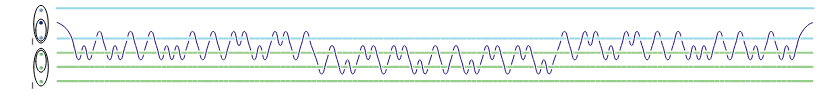
\includegraphics[width=\textwidth]{images/Cnot-weave-clean.png}
  \caption{A CNOT weave. From \cite{simon_topological_2006}}.
  \label{fig:weave}
\end{figure}
%Here, the identiy braid serves as an "Injector" of weaves of the same quantum number $q$, as seen in the CNot weave below.

\subsection{Outlook}

Theoretically, we now have a well-defined, topologically protected model of Tqc. However, as of 2024 there is no experimental evidence of finding anabelian anyons, specifically Majorana zero mode anyons (Ising), and most claims have been retracted \cite{gazibegovic_retraction_2022} \cite{castelvecchi_evidence_2021}. Recent claims such as \cite{pikulin_protocol_2021} are also not widely accepted. However, the existence of abelian anyons is mostly considered as fact \cite{glidic_signature_2024}. Most experimental approaches are done using the Quantum Hall Effect at $v = 2 / 5$.



\printbibliography




%\appendix
%\label{Appendix}


%\section{Homotopy group}

%A homotopy equivalence between any two spaces $X$ and $Y$ is given, if there is a pair of morphisms $X \to Y$ and $Y \to X$ such that both commute to the identity maps of the respective space. Two such spaces are also called {\it contractible}

%A homotopy between two continuous functions $f,g : X \to Y$ is a continuous interpolation $h : X \times [0,1] \to Y$. If this homotopy exists, $f$ and $g$ are homotopic. Equivalently, two loops are homotopic if they can be continuously deformed without leaving or breaking the space. Now, the {\it first homotopy group}, denoted by $\pi_1 (X,x_0) = \{ [\gamma] : \gamma \in \Omega(X,x_0)\}$

%This relates to the behaviour of anyons, as the configuration space in $\R^2$ is 

%\[
%  Conf_N(\R^2) = \{(x_1,x_2, \ldots ,x_n  ) \in (\R^2)^n %\mid x_i \neq x_j \forall i \neq j  \}
%\]

%The symmetric Group $S_n$ gives the Group action $S_n \times C_{n}(X) \to C_n(X)$

%Applying braids on a series of points gives a permutation of those points inducing a surjection $B_n \to S_n$. The set of braid operations that return to their original configuration is called the {\it pure braid group} $PB_n$ and is given by $\ker({B_n \to S_n})$. Further, this means that the symmetric group on $n$ covers the Braid group on $n$ strands. This entails a "linear" representation of the symmetric group in the braid group, whose group action can be seen as the concatenation of two braids elements over time.

%\section{Pentagon and Hexagon math}

%\begin{figure}[h ]
%  \centering
%  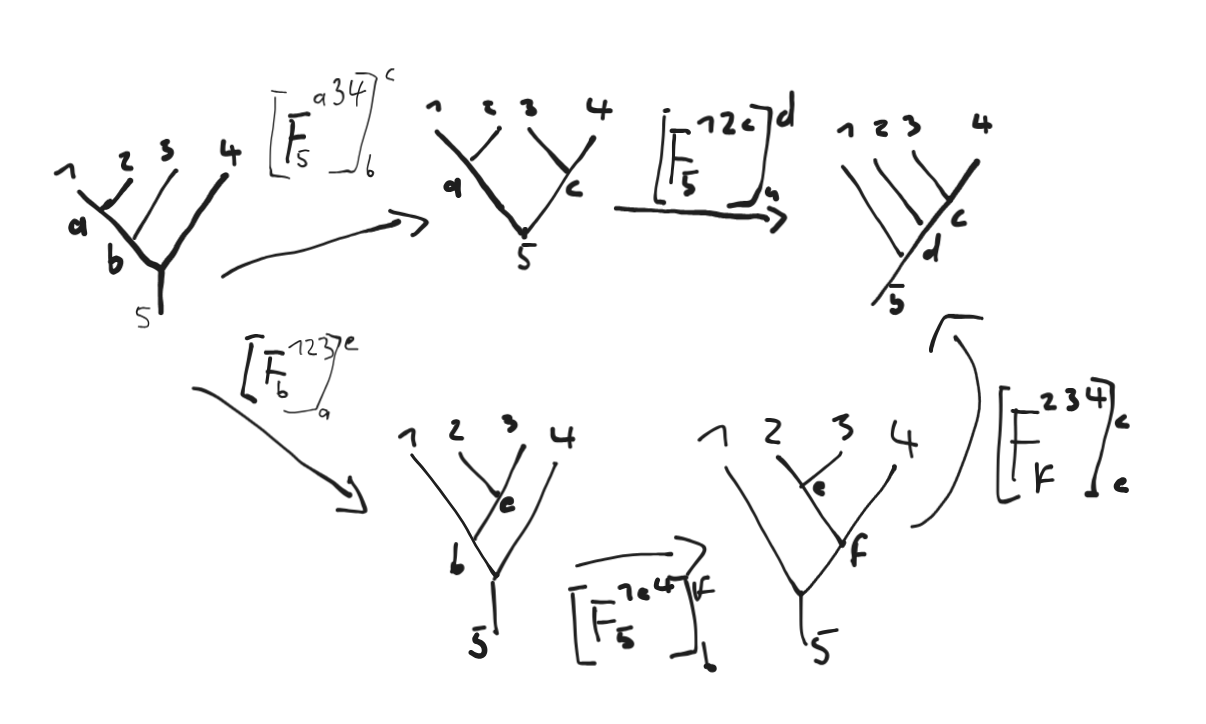
\includegraphics[width=0.8\textwidth]{pentagon_diagram.png}
%  \caption{The pentagon equation shown diagrammatically. Normally, we would have sums over all target fusions (so c, d, f) but we can just fix those and ignore them}
%  \label{fig:}
%\end{figure}

%Note on calculation: The only nontrivial $F$s in the anyonic category are $[F^{\tau \tau \tau}_{0}]_{\tau}^{\tau}$ and $F^{\tau \tau \tau}_{\tau}$.  Then we necessarily know $F^{3\tau}_{\tau}]_{0 0} = \frac{1}{\phi}$ and thus by unitarity $\left\vert b  \right\vert ^2 = \left\vert c  \right\vert^2 = 1 - \frac{1}{\phi^2}$

\end{document}  


%@misc{solovay_email,
%	author = {Solovay, Robert M.},
%	howpublished = {email},
%	title = {},
%	year = {1995}
%}